\documentclass[a4paper,UTF8]{article}
\usepackage{ctex}
\usepackage[margin=1.25in]{geometry}
\usepackage{color}
\usepackage{graphicx}
\usepackage{amssymb}
\usepackage{amsmath}
\usepackage{amsthm}
%\usepackage[thmmarks, amsmath, thref]{ntheorem}
\theoremstyle{definition}
\newtheorem*{solution}{Solution}
\newtheorem*{prove}{Proof}
\usepackage{multirow}
\usepackage{url}
\usepackage{enumerate}
\usepackage{listings}
\usepackage{caption}
\usepackage{subfigure}
\usepackage[colorlinks,linkcolor=black, anchorcolor=black,citecolor=black,]{hyperref}


\begin{document}
\title{\textbf{《计算机图形学》系统报告}}
\author{学号:181860077 姓名:佘帅杰,\href{mailto:3121416933@qq.com}{3121416933@qq.com}}
\maketitle

\section{综述}
基本完整的实现了所有需要的任务,同时附加实现了部分的拓展功能
\subsection{基本要求}
\begin{enumerate}
    \item 熟悉实验框架和所需的PyQt5知识
    \item 实现了所有的绘图算法,包括直线绘制,多边形绘制,椭圆和曲线绘制
    \item 实现了所有的图元操作算法,包括旋转,平移,缩放,裁剪
    \item 在GUI里对各个事件进行处理,使用核心算法模块中的算法绘制图元或者是对图元进行操作
    \item 实现了保存图元,设置画笔,重置画布等GUI标配功能
\end{enumerate}
\subsection{拓展功能}
\begin{enumerate}
    \item 实现了使用鼠标直接选中图元的操作,同时选中对象和右侧的列表一致
    \item 实现了编辑器里实用的复制和粘贴功能,便于系统的使用
    \item 有了对系统的编辑和使用,自然少不了手抖画错了,因此增加了删除功能,删除画错的部分
    \item 在反复的操作过程中自然需要方便快捷的快捷键,对应的也进行了实现包括复制粘贴等功能在内的对应快捷键
\end{enumerate}

\section{实验框架阅读和理解}
在实现之前自然要对拿到手的框架代码进行阅读和分析,可以显然的看到代码
主要都分布在三个文件中,分别进行阅读和分析
\subsection{cg\_algorithm.py}
这个文件主要就是实现绘图代码的算法,每一个函数基本都代表这一个需要
实现的功能或者是算法,每一个函数接受绘图所必须的点,一般都是以列表的
形式给出,其他的参数一般就是一些可选参数(如:想要实现的后台算法种类)
这一块结构比较简单,也是实现的核心和重点
\subsection{cg\_cli.py}
cli文件主要是负责解析命令行文件,并做出回应。基本的功能就是按行读取文件
然后利用split分解命令行,并根据预设的指令的格式进行匹配并执行\\\\
整体的主要代码逻辑如下
\begin{enumerate}
    \item 收到的是绘图的指令,那就使用特定的格式,把绘图的
    要求以及颜色等信息都保存在字典里,等待后续的使用。
    \item 收到的是saveCanvas指令,就会
    遍历先前提到的字典,对每一项进行解析,利用存储的信息调用对应的绘图算法
    得到像素点的坐标列表,根据坐标点的位置信息在画布数组上填入颜色信息(坐标
    信息实际上就是画布数组的下标信息)
    \item 收到的是resetCanvas指令,相对就会比较简单,就只需要重新设置
    画布的规格(高,宽)然后清空刚才提到的对象列表
\end{enumerate}
\subsection{cg\_GUI.py}
本模块就是对于之前的一些功能的集成,并对外提供图形化的界面进行使用。
基本的模块由三块构成
\begin{enumerate}
    \item MyItem继承于QGraphicsItem,本质上就是用来描述图元的类,保存了图元相关的信息,可以类比到Cli
    文件里的那个字典里的元素,只不过这里使用了一个专门的类来描述,同时由于有了图形化界面,
    所以对图元的描述又多了一个选中的标志位。以及图元的共性操作:上色显示。还有的就
    是一些不同图元的特色操作,如:选中框显示。
    \item MyCanvas继承于QGraphicsView,类比起来就是电视机的显示屏幕,负责图元的管理和显示,简单的可以类比
    做CLi里的那个字典保管着若干图元。但是对于GUI而言还有鼠标等事件的Handle,所以对应的这个模块负责了
    鼠标在画布上的操作的处理,以及对应的对图元进行处理,如绘制,选中等等。刚好前文说到,他保管着所有
    图元的信息字典。
    \item MainWindow继承于QMainWindow,负责的区域是除了画布以外的窗口区域,也就是菜单等
    所以他负责构造整个菜单的结构以及按钮,还有就是绑定菜单信号和对应处理信号的槽函数,但是
    他是负责菜单,不直接的对画布和图元操作,因此二者时间的通信实际上是通过设置State来做到的。
    对应的MyCanvas在处理鼠标事件的时候也会根据状态的不同做出改变。(比如说,菜单选中了"选择图元",则
    MainWindow把状态设置为"Selecting",这个时候再用鼠标点击画布等操作,MyCanvas就会根据Selecting这个
    状态对对应的鼠标事件进行处理。)
\end{enumerate}

\section{算法介绍}
\subsection{直线绘制算法}

\subsubsection{Naive}
\paragraph{算法原理} 
Naive算法相对简单,算法的基本思路如下:
\begin{itemize}
    \item [(1)] 
    首先排除可能的特殊情况,即横坐标为0斜率不存在情况,然后直接计算对应的(x,y)坐标组合
    \item [(2)]
    没有触发特殊情况则计算斜率,斜率即X轴方向增大的时候Y对应的增量
    \item [(3)]
    然后就横坐标移动,纵坐标做对应的变化
  \end{itemize}


\paragraph{算法评估} 
对Naive算法性质简单评估
\begin{enumerate}
    \item 优点:简单易懂便于理解,符合数学公式
    \item 缺点:算法每生成一个点都需要做一次乘法和若干次的加法和减法,复杂度较高
\end{enumerate}

\subsubsection{DDA}
\paragraph{算法原理}
DDA算法\\
DDA算法,也就是数字差分分析方法,利用计算两个坐标方向的差分来确定线段显示的屏幕像素
位置的线段扫描转化算法,也就是说对一个坐标轴上以单位时间间隔对线段采样($\Delta x=1$ 或 $\Delta y=1$)
,计算$\Delta y$ 或$\Delta x$决定另一个坐标轴上最靠近线段的路径的对应整数值\cite{ref1}

DDA算法实际上也可以看作是在沿着某一条坐标轴做扫描,只不过基于斜率的不同导致了扫描的坐标轴不同
原因:如果都是按照Naive那样沿着X轴进行扫描进而得到所谓的Y轴的位置,那么对于斜率大的直线而言,
由于斜率大导致Y轴步长远大于X轴的步长,进而导致了线上的点非常的稀疏,所以DDA采用的是根据斜率的值
来动态的选择沿着哪一条轴扫描。需要注意的是,由于沿着Y轴扫描的时候,X轴上的增量就不再是斜率,而是斜率的倒数

\begin{figure}[h]
	\centering
	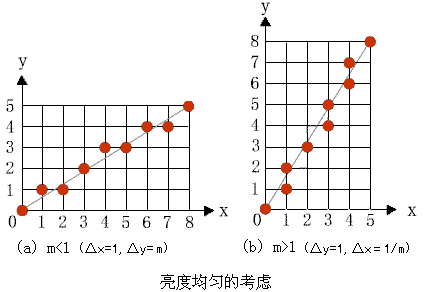
\includegraphics[scale=1]{figure/DDA.png}
	\caption{DDA算法示意图}
	\label{fig:DDA}
\end{figure}

如图\ref{fig:DDA},有如下公式

$$
\begin{cases}
    y_{k+1}=y_k + m \quad \text{$m<=1$}\\
    x_{k+1}=x_k + \frac{1}{m} \quad \text{$m>1$}
\end{cases}
$$
算法的测试如下:在GUI中沿着各种方向画线并观察\\
\begin{figure}[h]
	\centering
	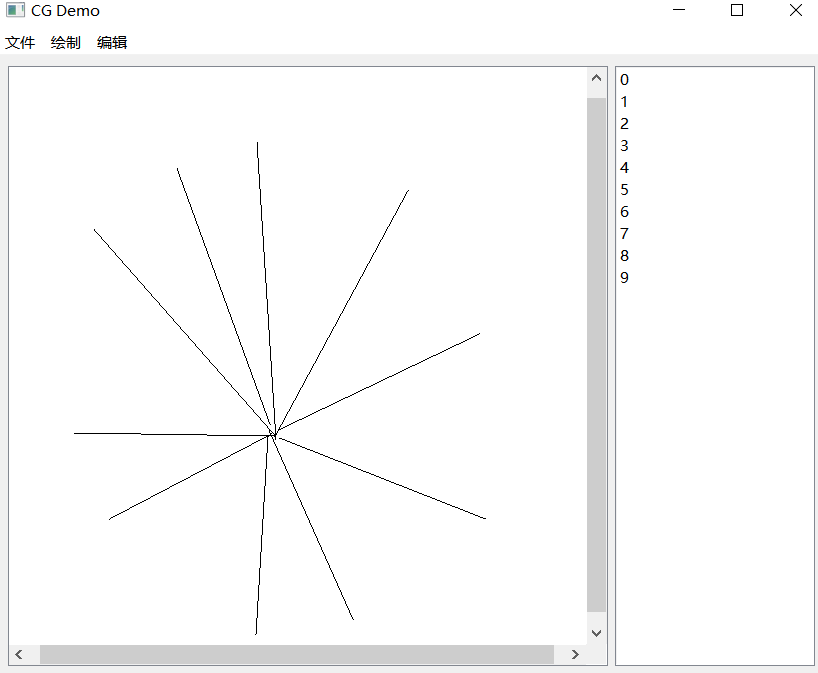
\includegraphics[scale=0.4]{figure/DDA_GUI.png}
	\caption{DDA\_GUI测试示意图}
	\label{fig:DDA_GUI}
\end{figure}

\paragraph{算法评估} 
基于上述的原理对DDA算法性质简单评估
\begin{enumerate}
    \item 优点:DDA算法的计算是增量计算(充分的利用了光栅的特性),每一次计算都是充分的利用了上一次的计算结果,
    所以DDA算法的复杂度小于之前的Naive算法(基于直线方程的)
    \item 缺点:浮点数操作会导致误差的积累,使得结果偏离路线
    \item 缺点:取整和浮点数操作仍然耗时,可以分解增量$\frac{1}{m}$ 和$m$ 为整数和小数,使得计算为整数间的计算而提高效率
\end{enumerate}


\subsubsection{Bresenham}
\paragraph{算法原理}
Bresenham算法\\
Bresenham算法是一种精准而有高效的光栅线段生成算法,他可用于圆和其他曲线显示
的整数增量运算,简单的说就是仍然是选定了一个扫描的方向,然后沿着方向进行扫描,但是
在扫描的过程中对另一个坐标的像素进行选择\\
为了简化像素的选择,Bresenham算法通过引入整形变量去衡量候选像素和实际像素的偏移
并利用对整形变量符号的检测来决定最接近真实路径的像素。\\
\begin{figure}[h]
	\centering
	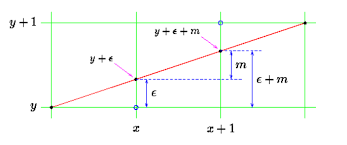
\includegraphics[scale=1]{figure/bresenham.png}
	\caption{Bresenham算法示意图}
	\label{fig:Bresenham}
\end{figure}\\
真实位置$y=mx_{k+1}+b=m(x_k+1)+b$\\
候选像素也就是$y_{k+1}$和$y_k$\\
那么就计算二者的误差(距离差)得到如下的公式
$$
\begin{cases}
    d{1}=y-y_k = m(x_k+1)+b-y_k \\
    d{2}=y_{k+1}-y =y_{k+1}- m(x_k+1)+b
\end{cases}
$$
由于需要比较二者的大小,于是很自然的对二者进行做差
即如下公式\\
\indent $ d{1}-d{2}=2m(x_k+1)-2y_k+2b-1$\\
基于上述的公式得到本算法的核心:决策变量\\
\indent $p_k=\Delta{x}(d_1-d_2)=2\Delta{y}x_k-2\Delta{x}y_k+c$\\
本公式的核心还是在于两个候选像素的误差大小比较(作差)。前面乘上的
$\Delta{x}$主要还是为了优化计算为整数之间的计算而提高效率。
同时$c=2\Delta{y}+\Delta{x}(2b-1)$是一个常量,并会在增量计算中
被忽略
很显然在绘图的时候应该选择误差小的,也就是$p_k$的正负性可以很清楚的
作为像素决策的依据\\\\
目前问题就被转化为如何去计算每一步的$p_k$作选择的依据\\
$p_{k+1}-p_k=2\Delta y x_{k+1}(x_{k+1}-x_k) -2\Delta x( y_{k+1}-y_k)$\\
经过化简之后就可以得到\\
$p_{k+1}=p_k+2\Delta y-2\Delta x( y_{k+1}-y_k)$\\
$$
\begin{cases}
    y_{k+1}-y_k=1 \quad \text{$p_k>0$}\\
    y_{k+1}-y_k=0 \quad \text{$p_k<0$}
\end{cases}
$$
个人的理解就是如\ref{fig:Bresenham}中所示,就是误差的积累
当误差达到一定的大小的时候就只能够去选择下一步的$y_k$,也就是在选择之后需要重新的计算
误差,类似于加法加到一定大小之后取模的操作\\
经过上述的分析之后,很容易就可以得到此算法的工作流程\\
\begin{itemize}
    \item [(1)] 
    计算常量值$\Delta{x}$, $\Delta{y}$, $2\Delta{y}$, $2\Delta{y}-2\Delta{x}$
    \item [(2)]
    循环扫描,对$p_k$的值进行判断
    \item [(3)]
    若$p_k$的值为正,则y加1,同时$p_k=2\Delta{y}-2\Delta{x}$
    \item [(3)]
    反之若$p_k$的值为负,则y不变,同时$p_k=2\Delta{y}$
\end{itemize}

在GUI中测试:\\

\begin{figure}[h]
	\centering
	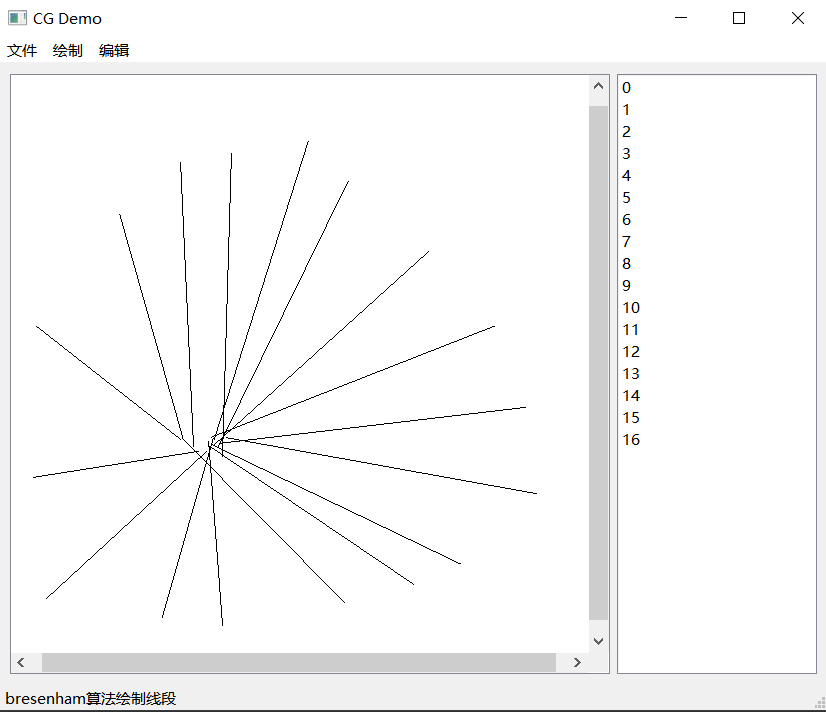
\includegraphics[scale=0.4]{figure/Bre_GUI.png}
	\caption{Bre\_GUI测试示意图}
	\label{fig:Bre_GUI}
\end{figure}

\paragraph{算法评估} 
基于上述的原理对Bresenham算法性质简单评估
\begin{enumerate}
    \item 优点:计算量进一步的减小,每一次的计算都只发生的整数之间,并且都是
    复杂度相对较低的加减法计算,同时只需要判断决策参数的符号,算法效率得到提高
    \item 优点:可以利用并行计算加快图像生成速度
    \item 缺点:稍微复杂,直接看公式可能不能很好的理解
\end{enumerate}

上述的算法大多都经过了在GUI环境下的测试,于是选择在
命令行环境下进行统一测试,分析结果。
整合测试:对上述的三个直线生成代码进行测试,为了方便直接在cli中使用文件测试:\\\\
测试语句如下\\
\indent resetCanvas 600 500\\
\indent setColor 0 0 255\\
\indent drawLine line1 195 363 316 50 Naive\\
\indent setColor 0 255 0\\
\indent drawLine line3 190 343 311 30 DDA\\
\indent setColor 255 0 0\\
\indent drawLine line2 185 323 305 10 bresenham\\
\indent saveCanvas 3\\

测试结果如下\\
\begin{figure}[h]
	\centering
	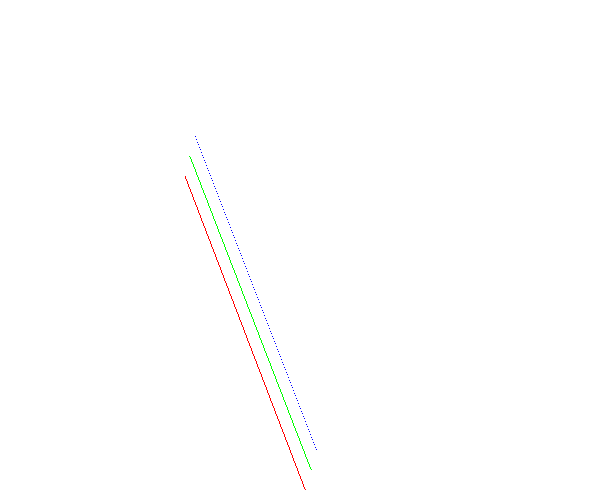
\includegraphics[scale=0.6]{figure/linetest.png}
	\caption{直线绘制算法测试示意图}
	\label{fig:line}
\end{figure}

\subsection{多边形绘制算法}
对于多边形的绘制,本质上就是绘制多条直线,所需要做的就是在顶点之间绘制
直线,进而形成图形的边界。所以本身并不涉及过多的算法实现,只需要在命令行和GUI功能中加上代码,链接
上对应的功能实现就可以\\
分别对Cli和GUI文件进行更改\\

测试输入:\\
\indent resetCanvas 600 500\\
\indent setColor 0 0 255\\
\indent drawPolygon line5 215 353 365 353 365 453 215 453 bresenham\\
\indent drawPolygon line6 235 373 385 373 385 473 235 473 DDA\\
\indent saveCanvas 3\\

测试结果如下\\
\begin{figure}[h]
	\centering
	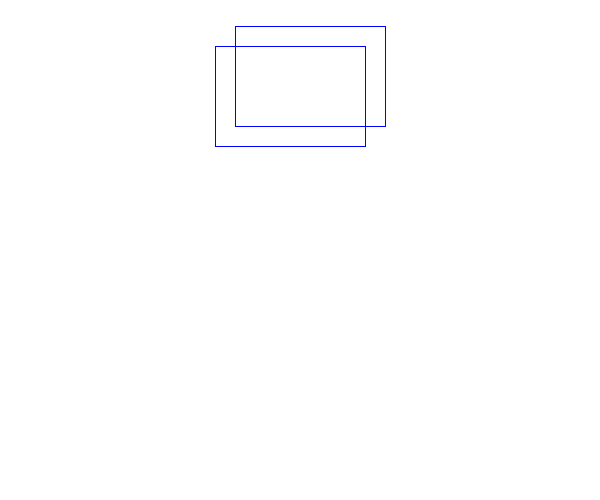
\includegraphics[scale=0.6]{figure/polytest.png}
	\caption{多边形绘制算法测试示意图}
	\label{fig:Poly}
\end{figure}


%   %
\subsection{中点圆绘制算法}
\paragraph{算法原理}
中点圆算法\\
首先,椭圆(或者说圆)有若干的性质:
\begin{itemize}
    \item 高度的对称性,也就是只需要生成一部分就可以得到整体
    \item 斜率不断的动态变化,斜率不唯一
\end{itemize}
中点圆算法的原理实际上和Bresenham算法的原理相似,都是通过某一个方向的
扫面,在另一个方向上的候选里去评估错误率,然后进一步的选择哪一个像素点
不同之处就在于所谓的椭圆方程。针对先前已经实现的算法不难发现,这种针对
一个方向扫描的算法的问题就在于用哪个方向,最后的答案往往是根据斜率来决
定,同样的在椭圆这里,由上述的性质知道椭圆绘制需要分段\\
进而计算得到了分段点:\\
\indent $2r_y^2>=2r_x^2y$\\
即这里作为分界分段求解
同时对于段内,需要同样的要引入一个决策变量\\
$p_k=F(x_{k+1},y-\frac{1}{2})=(x_k+1)^2+(y_k-\frac{1}{2})^2-r^2$\\
同理的利用决策变量的符号来决定另一个坐标轴的移动,这个变量表示着候选
像素中点的是否在圆内,也就是标识了所谓的候选点的质量。推导得到了这个决策
变量的增量计算公式如下:\\
区域一:
$$
\begin{cases}
    p_{k+1}=p_k +2r_y^2x_k+3r_y^2 \quad \text{$p<0$}\\
    p_{k+1}=p_k +2r_y^2x_k+3r_y^2-2r_x^2y_k+2r_x^2 \quad \text{$p>=0$}
\end{cases}
$$
区域二:
$$
\begin{cases}
    p_{k+1}=p_k -2r_x^2y_k+3r_x^2 \quad \text{$p<=0$}\\
    p_{k+1}=p_k +2r_y^2x_k+3r_x^2-2r_x^2y_k+2r_y^2 \quad \text{$p>0$}
\end{cases}
$$\\
并根据公式计算决策变量的初始值\\\\
$p_0=r_y^2-r_x^2r_y+\frac{r_x^2}{4}$\\\\
算法的整体流程即如下
\begin{itemize}
    \item [(1)] 
    计算决策变量的初始值,并选择椭圆最上方的点
    \item [(2)]
    沿着X轴循环扫描,根据公式更新决策变量和y值,直到结束区域一
    \item [(3)]
    记忆区域一的最后一个位置,根据公式计算新的决策变量初始值
    \item [(4)]
    沿着Y轴循环扫描,根据对应公式计算决策变量和x值,直到结束区域二
    \item [(5)]
    由先前得到的第一象限的全部图像做图形变化,得到完全椭圆
    \item [(6)]
    根据真实图像所在中心,平移现图像至真实位置结束算法
  \end{itemize}
测试输入:\\
\indent resetCanvas 600 500\\
\indent setColor 0 0 255\\
\indent drawEllipse line7 0 0 200 200\\
\indent drawEllipse line8 100 100 300 300\\
\indent saveCanvas 3\\
测试结果如下(见图\ref{fig:circletest})
\begin{figure}[h]
	\centering
	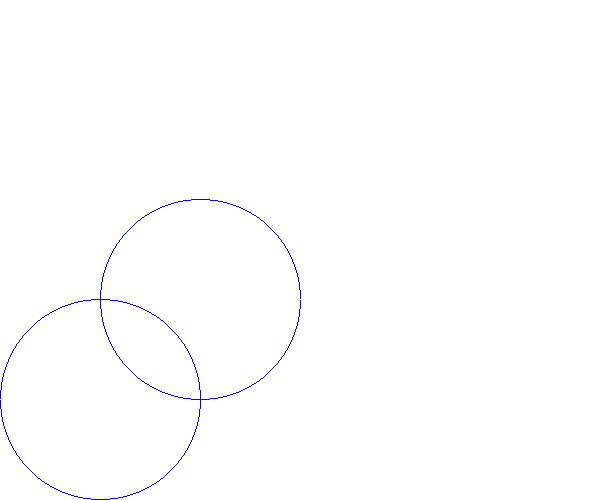
\includegraphics[scale=0.3]{figure/circletest.png}
	\caption{中点圆绘制算法测试示意图}
	\label{fig:circletest}
\end{figure}\\


\subsection{算法正确性检查模块}
\subsubsection{图片读取}
基本步骤如下(详细可见代码:Score\_Test.py)

\begin{itemize}
    \item [(1)] 
    利用os读取到对应图片目录下的所有的文件名字
    \item [(2)]
    拼接得到最终的路径名
    \item [(3)]
    使用PIL库对图片进行读取RGB
    \item [(4)]
    使用Numpy库对数据统一转化为Array
  \end{itemize}

\subsubsection{校验算法}
使用多种方法对多种算法实现的最后结果进行对比和分析\\
(注:仅在本文件为了实现的方便调用了sklearn用于计算余弦相似度。
整个工程的其他位置的代码没有使用任何未经允许的库,如果这也不合规则
也可删除sklearn的调用)
\begin{itemize}
    \item 像素级别对比和差异统计:使用numpy特性扫描图片,
    计算有效区域(即作图区域,可以避免由于作图部分过于稀疏导致的结果差异)
    以及差异区域,计算差异度
    \item 图片整体的相似度计算,利用RGB值对整个图片建模表示,然后计算余
    弦相似度以统计计算图片之间的差异,设置一定的阈值进行警示可能的作图错误
\end{itemize}
如下为一次测试的样例\\

\begin{figure}[h]
	\centering
	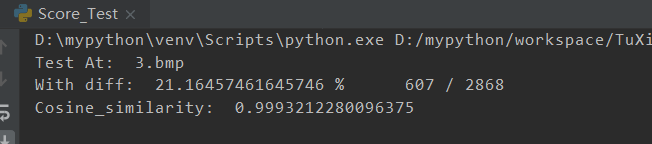
\includegraphics[scale=0.6]{figure/test.png}
	\caption{Score校验算法}
	\label{fig:Score}
\end{figure}
如图\ref{fig:Score},差异度的计算方式为差异度=差异区域像素点数目/着色像素点数目\\
同时计算两个图片向量的余弦相似度作为参考\\
(简单的经验:99.9+\%代表良好,低于99.9\%则可能存在算法绘图错误)\\
\subsection{GUI功能加强}
在GUI方面,为了方便使用加入了使用鼠标直接选中图元的操作
由原框架代码可以知道,选中图元可以通过界面右侧的列表,根据编号选中图元,即选中图元的基本操作
已经被实现,但是由于图元和编号并不显式绑定,所以考虑使用鼠标更加便捷直观的选中图元,对应的就是
需要在鼠标按下和释放的时候,根据当前的状态判断是不是在选中图元的状态。如果是则根据当前的鼠标位置
计算对应选中的图元,然后执行切换选中的过程,后半部分可以通过调用原框架代码的时候达到代码统一化
简洁化的目的\\
基本的实现流程如下

\begin{itemize}
    \item [(1)] 
    利用菜单键进入"Selecting"状态
    \item [(2)]
    在画布界面中点击所需的图元
    \item [(3)]
    鼠标的点击和释放触发信号,并发现当前处于"Selecting"状态,计算得到当前的图元
    \item [(4)]
    如果先前选中图元,则清除先前的选中
    \item [(4)]
    设置当前的选中状态,刷线画布状态,此时后续的处理则会使得图元被红色矩阵包围,显示为选中状态
  \end{itemize}

  \begin{figure}[htbp]
    \centering    %居中
     
    \subfigure[菜单选择] %第一张子图
    {
        \begin{minipage}{7cm}
        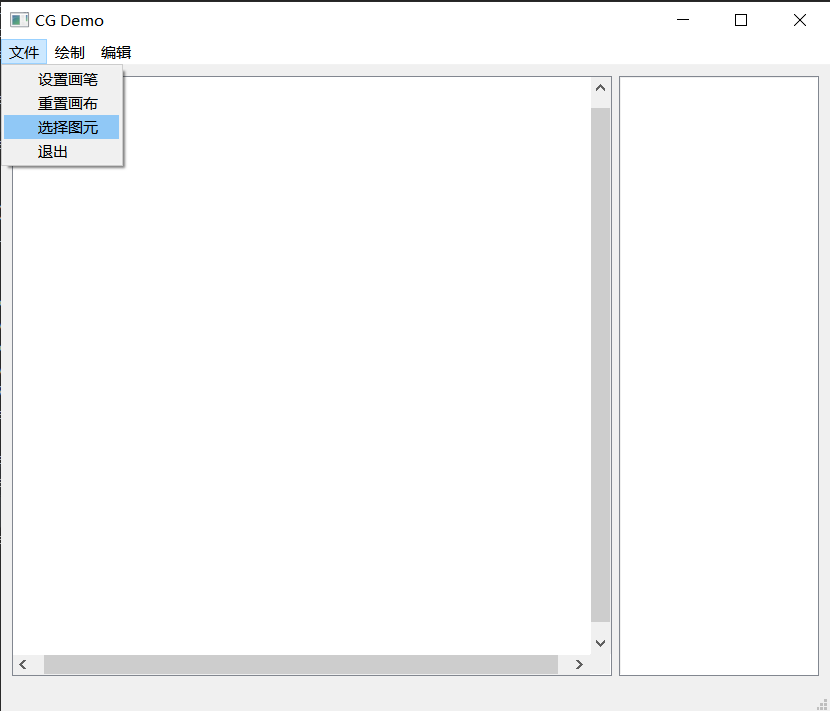
\includegraphics[scale=0.2]{figure/choose.png}   %以pic.jpg的0.5倍大小输出
        \end{minipage}
    }
    \subfigure[鼠标选中] %第二张子图
    {
        \begin{minipage}{7cm}
        \centering      %子图居中
        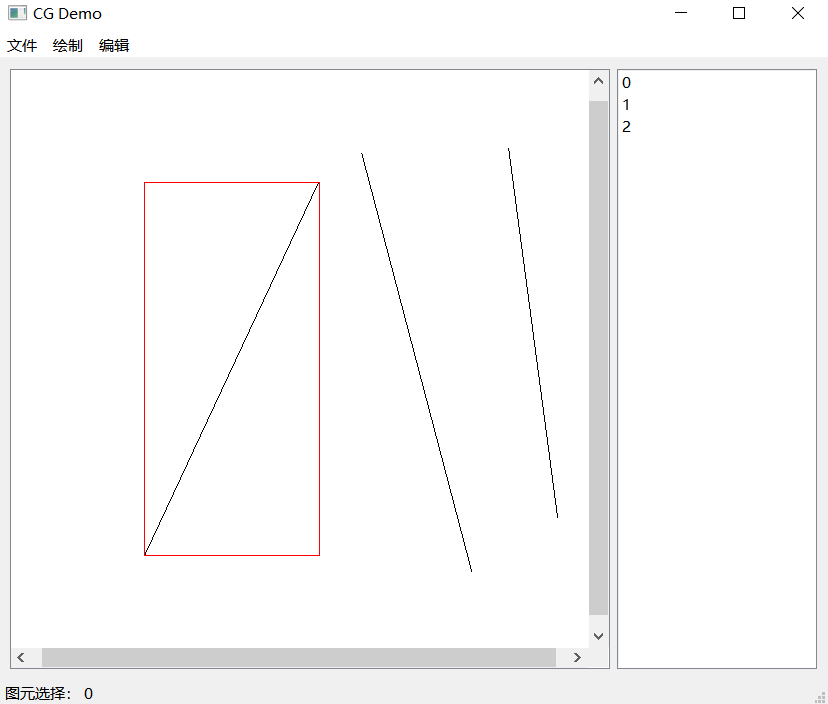
\includegraphics[scale=0.2]{figure/choose2.png}   %以pic.jpg的0.5倍大小输出
        \end{minipage}
    }
     
    \caption{鼠标选中图元测试实例} %  %大图名称
    \label{fig:1}  %图片引用标记
\end{figure}

\subsection{曲线的参数化表示}
在绘制曲线之前,首先需要了解怎么对曲线进行参数化的表示
实际上对于表示一条曲线的各个变量,都可以用某个参数的函数来表示
$$
\begin{cases}
    x=x(u)\\
    y=y(u)\\
    z=z(u)
\end{cases}
$$

三个坐标分量就组成曲线上该点的位置矢量,曲线就可表示为参数u的矢函数
通过这个对曲线进行参数化表示,也是后面绘制曲线的算法的重要基础
对应的图元的生成就可以看作是这个联结的变量的变化过程

\subsection{Bezier曲线绘制算法}
一阶的Bezier曲线就是一条直线,相当于是在两个控制点之间做插值,最后相当于是一个点在两个点之间移动。
最后他的轨迹就是一条直线,也就是两个控制点之间的曲线。这个过程使用公式可以表达为:$ B_{1}(t)=P_0+(P_1-P_0) t$。这里的t可以和上文的
曲线参数化表示关联,t就是那个负责联结的参数。
对于有三个控制点的情况,这个时候是二阶的Bezier曲线,可以看作是两层的一阶Bezier曲线,基本的理解方式可以看到下面的图

\begin{figure}[h]
	\centering
	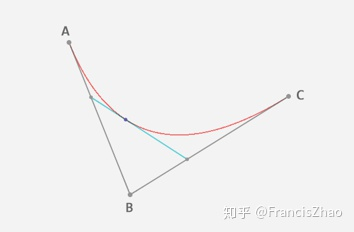
\includegraphics[scale=0.8]{figure/b.png}
	\caption{二阶Bezier算法理解图}
	\label{fig:bezier-alg}
\end{figure}

上述的图可以看出整个过程还是一个插值的过程,在一次插值的结果的基础上做了第二次插值得到结果
同理的更加高阶的Bezier都能够一步一步的降阶
整个过程还可以发现到系数是二项式的展开,进而得到公式实现算法。\\

$$f(x)=
\begin{cases}
    P_{i}  \\
    (1-u)P_{i}^{r-1}+(1-u)P_{i+1}^{r-1}
\end{cases}
$$
对应的图片
\begin{figure}[h]
	\centering
	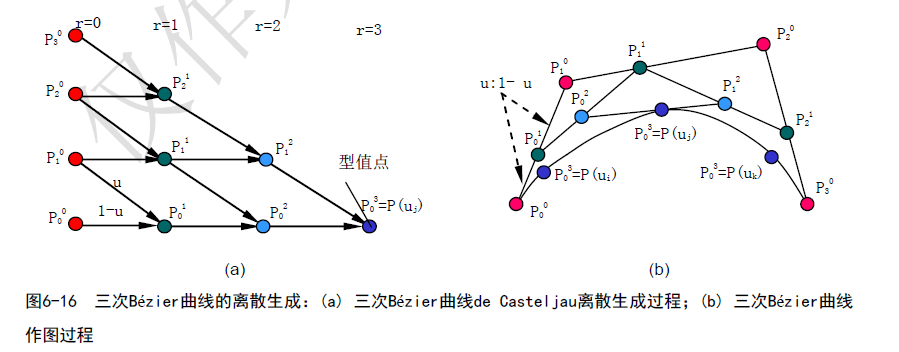
\includegraphics[scale=0.6]{figure/bezier2.png}
	\caption{Bezier算法演示图}
	\label{fig:bezier2}
\end{figure}

算法使用过的指令文件:\\

resetCanvas 600 600\\

setColor 0 255 0\\

drawCurve curve1 50 200 100 100 150 200 Bezier\\

drawCurve curve2 50 400 100 300 150 400 200 300 Bezier\\

saveCanvas 5\\

算法结果:\\
\begin{figure}[h]
	\centering
	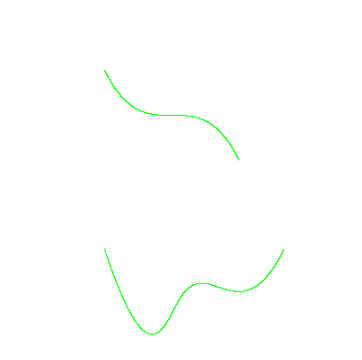
\includegraphics[scale=0.8]{figure/bezier.png}
	\caption{Bezier算法测试结果图}
	\label{fig:bezier-result}
\end{figure}

\subsection{B-spline曲线绘制算法}
\par B样条曲线算法涉及到了基函数:什么是基函数?
基函数 就是一个函数的固定形式,也就是函数只会在这个函数的基础上变化而不会丢掉的函数,在数学中,
基函数是函数空间一组特殊的基的元素。对于函数空间中的连续函数都可以表示成一系列基函数的线性组合,
就像是在向量空间中每个向量都可以表示成基向量的线性组合一样。
\par 同时由于Bezier算法本身的一些问题如:缺少局部性,不够灵活等等,所以B样条出现
虽然上面说了B样条有所不同,但是B样条的本质还是一个降阶然后解决问题的过程。
$$
P(t)=
\begin{bmatrix} 
    t^3 & t^2 & t & 1 
\end{bmatrix}
\begin{bmatrix} 
    -1 & 3 & -3 & 1 \\ 
    3 & -6 & 3 & 0 \\ 
    -3 & 0 & 3 & 1 \\ 
    1 & 4 & 1 & 0 \\ 
\end{bmatrix}
\begin{bmatrix} 
    p_0 \\ 
    p_1 \\ 
    p_2 \\ 
    p_3 \\ 
\end{bmatrix}
$$
基于上述的公式可以在四个控制点的三次B样条进行绘制曲线,但是在实际的情况里
控制点可能不止4个,对应的方法就是利用一个移动的窗口在控制点数组上滚动,举个例子就是
1,2,3,4,5,得到对应的窗口1,2,3,4和2,3,4,5。这样得到的曲线每一段
都能够自然衔接,同时具有连续性。下面的图也可以做辅助说明
\begin{figure}[h]
	\centering
	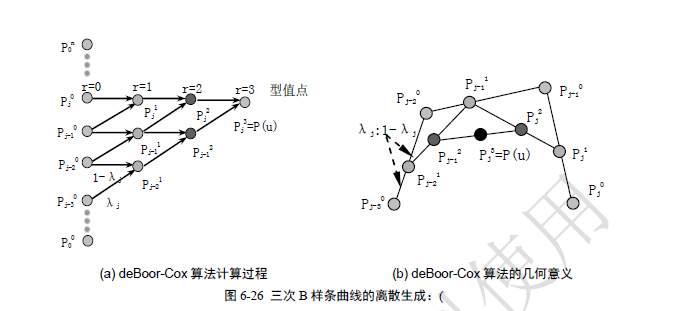
\includegraphics[scale=0.6]{figure/b-spline.png}
	\caption{B-spline算法示意图}
	\label{fig:b-spline-alg}
\end{figure}

实现之后使用算法进行测试,测试语句如下:\\

resetCanvas 600 600\\

setColor 0 0 255\\

drawPolygon polygon2 250 400 300 300 350 400 400 300 Bresenham\\

setColor 0 0 0\\

drawCurve curve3 250 400 300 300 350 400 400 300 B-spline\\

setColor 0 0 255\\

drawPolygon polygon3 250 200 300 50 350 250 400 100 450 200 Bresenham\\

setColor 0 0 0\\

drawCurve curve4 250 200 300 50 350 250 400 100 450 200 B-spline\\

saveCanvas 5\\

测试的结果如下
\begin{figure}[h]
	\centering
	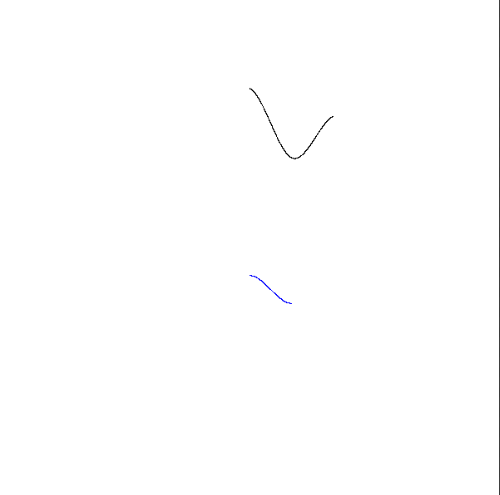
\includegraphics[scale=0.6]{figure/b-spline-result.png}
	\caption{B-spline测试结果图}
	\label{fig:b-spline-result}
\end{figure}

\subsection{图元平移算法}
平移严格的说是把一个点沿着直线路径从一个坐标位置移动到另一个坐标位置的重定位的
过程,说的简单的一些就是,图元的平移就是相对简单一些,图元的构造来源于传入的参数,即“控制点”
相对的,如果想要图元的位置进行平移,只需要对图元的控制点进行操作,
进行对应的平移,则最后的图形也会做对应的平移
算法的测试如下:使用如下的测试指令:\\

resetCanvas 600 600\\

setColor 0 255 0\\

drawLine line1 0 0 500 250 DDA\\

setColor 255 0 0\\

drawLine line2 0 0 500 250 Bresenham\\

translate line2 0 50\\

saveCanvas 1\\

测试的结果如下
\begin{figure}[h]
	\centering
	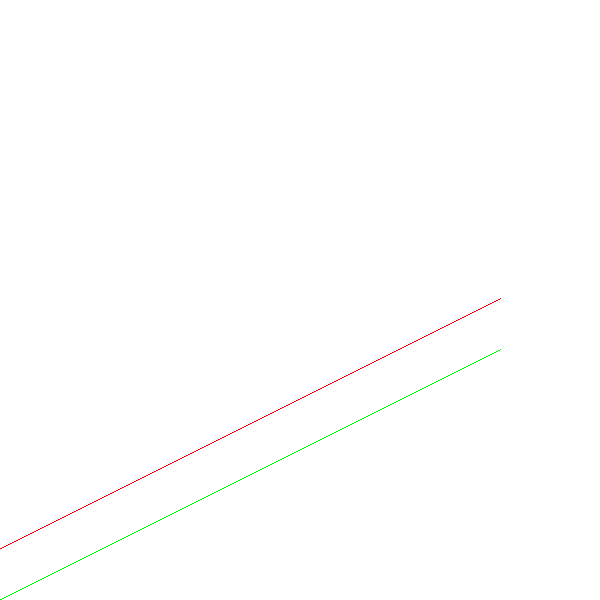
\includegraphics[scale=0.4]{figure/1.png}
	\caption{平移算法测试示意图}
	\label{fig:Rotate}
\end{figure}

\subsection{图元旋转算法}
旋转变化主要是二维的,就是把坐标点关于某个位置转动一个角度,然后确定新的坐标位置的
过程,对应也有公式可以进行参考,对应的公式参考如下:

\begin{figure}[h]
	\centering
	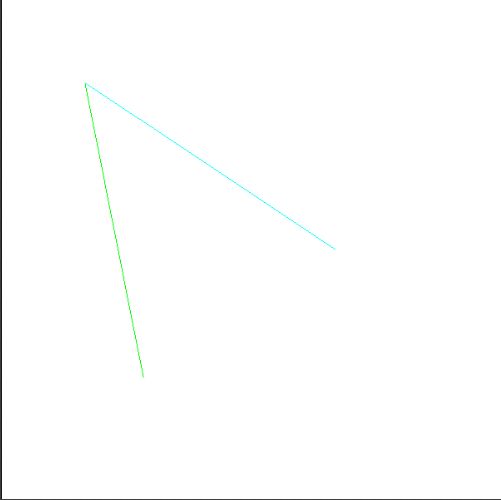
\includegraphics[scale=0.5]{figure/rotate.png}
	\caption{旋转公式图}
	\label{fig:rotate-alg}
\end{figure}

然后对应的对算法进行测试,使用的测试指令文件基本如下\\

resetCanvas 600 600\\

setColor 0 255 0\\

drawLine line1 100 100 400 300 DDA\\

setColor 0 255 255\\

drawLine line2 100 100 400 300 DDA\\

rotate line1 100 100 45\\

saveCanvas 1\\

\begin{figure}[h]
	\centering
	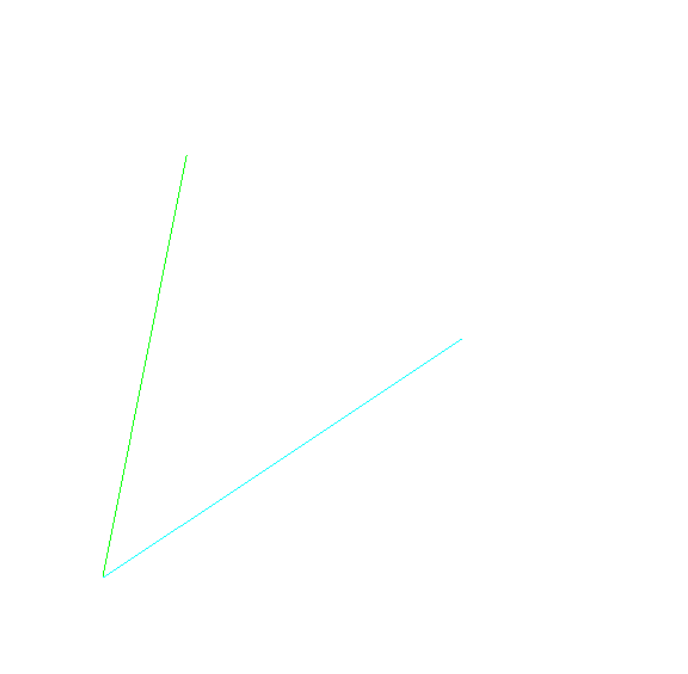
\includegraphics[scale=0.4]{figure/rotate_test.png}
	\caption{旋转算法测试结果图}
	\label{fig:rotate-result}
\end{figure}

\subsection{图元缩放算法}
同上所述,图元的构造主要来自于控制点的限制,对应的可以对控制点的位置进行修改,
缩放可以得到一个缩放的中心和倍数,对每一个控制点,查看其到缩放中心的位置,然后
把这个位置乘上缩放的倍数就可以很直观的看到,整个图形沿着缩放中心缩小或者是放大的
现象,这个算法相对也要简单一些

\begin{figure}[ht]
	\centering
	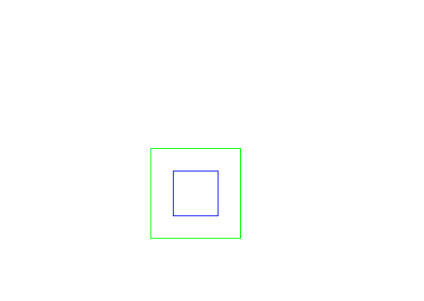
\includegraphics[scale=0.5]{figure/scale.png}
	\caption{缩放测试结果图}
	\label{fig:scale-alg}
\end{figure}

\subsection{图元裁剪算法}
识别图元在指定区域内外部的算法叫做裁剪,用来裁剪对象的区域被称为裁剪窗口。
当给定图元和裁剪窗口之后只留下(显示)给定的范围内的部分,而对于区域外的部分则
不予显示,
图元的裁剪算法很多,但是由于有很多的图元需要执行裁剪操作,对裁剪算法的效率有比较高的
要求
\subsubsection{Cohen-Sutherland算法}
这个算法的的基本思路就是对整个曲线进行了切分和分类,可以比较显示和可理解的
表示出一个线段和裁剪窗口之间的位置关系,对于完全在内部和外部的线段可以快速
判断而提高效率,编码的方式可见下图
\begin{figure}[h]
	\centering
	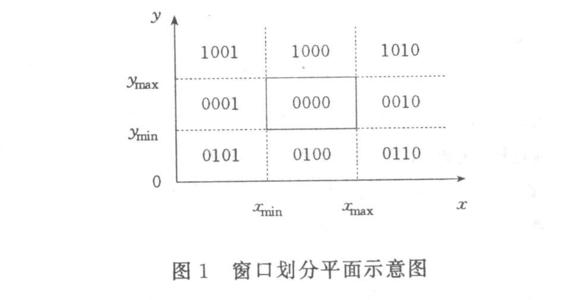
\includegraphics[scale=0.4]{figure/2.png}
	\caption{裁剪区域编码示意图}
	\label{fig:Rotate}
\end{figure}
然后可以直接通过比较或者是作差得到对应的区域码,对得到的两个区域码执行对应的计算
来判断直线和裁剪窗口的对应关系,比如说二者的区域码都是0000则说明整个线段都在裁剪
窗口里。或者是二者相与的结果不是0000,则说明整个线段都在区域外。\\
上述的两种情况是相对简单的两种,都不需要做相对复杂的操作,对于比较复杂度情况
就是有一部分的线在区域内,这就需要求解交点等操作,基本的思路就是求交点,然后确定
那一部分是要被丢弃的,然后在剩余的部分继续做求解\\
使用下述的指令文件进行测试:\\

resetCanvas 600 600\\

setColor 0 255 0\\

drawLine line1 0 0 500 250 DDA\\

setColor 255 0 0\\

drawLine line2 0 0 500 250 Bresenham\\

translate line2 0 50\\

clip line2 50 50 400 200 Cohen-Sutherland\\

drawPolygon polygon4 50 50 400 50 400 200 50 200 Bresenham\\

saveCanvas 1\\

对应的测试结果如下:\\

\begin{figure}[h]
	\centering
	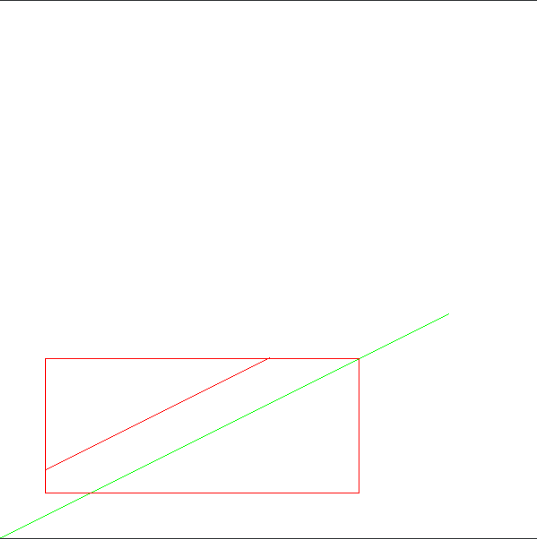
\includegraphics[scale=0.4]{figure/clip1.png}
	\caption{Cohen-Sutherland算法测试结果}
	\label{fig:Cohen-Sutherland算法剪切}
\end{figure}

\subsubsection{梁友栋-Barsky算法}
这个算法的最基本的思路把点和面都看作是大量的
点的集合,然后裁剪的结果就应该是二者的交集

类似的,这个裁剪算法也是用了一些参数来判断二者的相对的关系,基本的示意图如下
\begin{figure}[h]
	\centering
	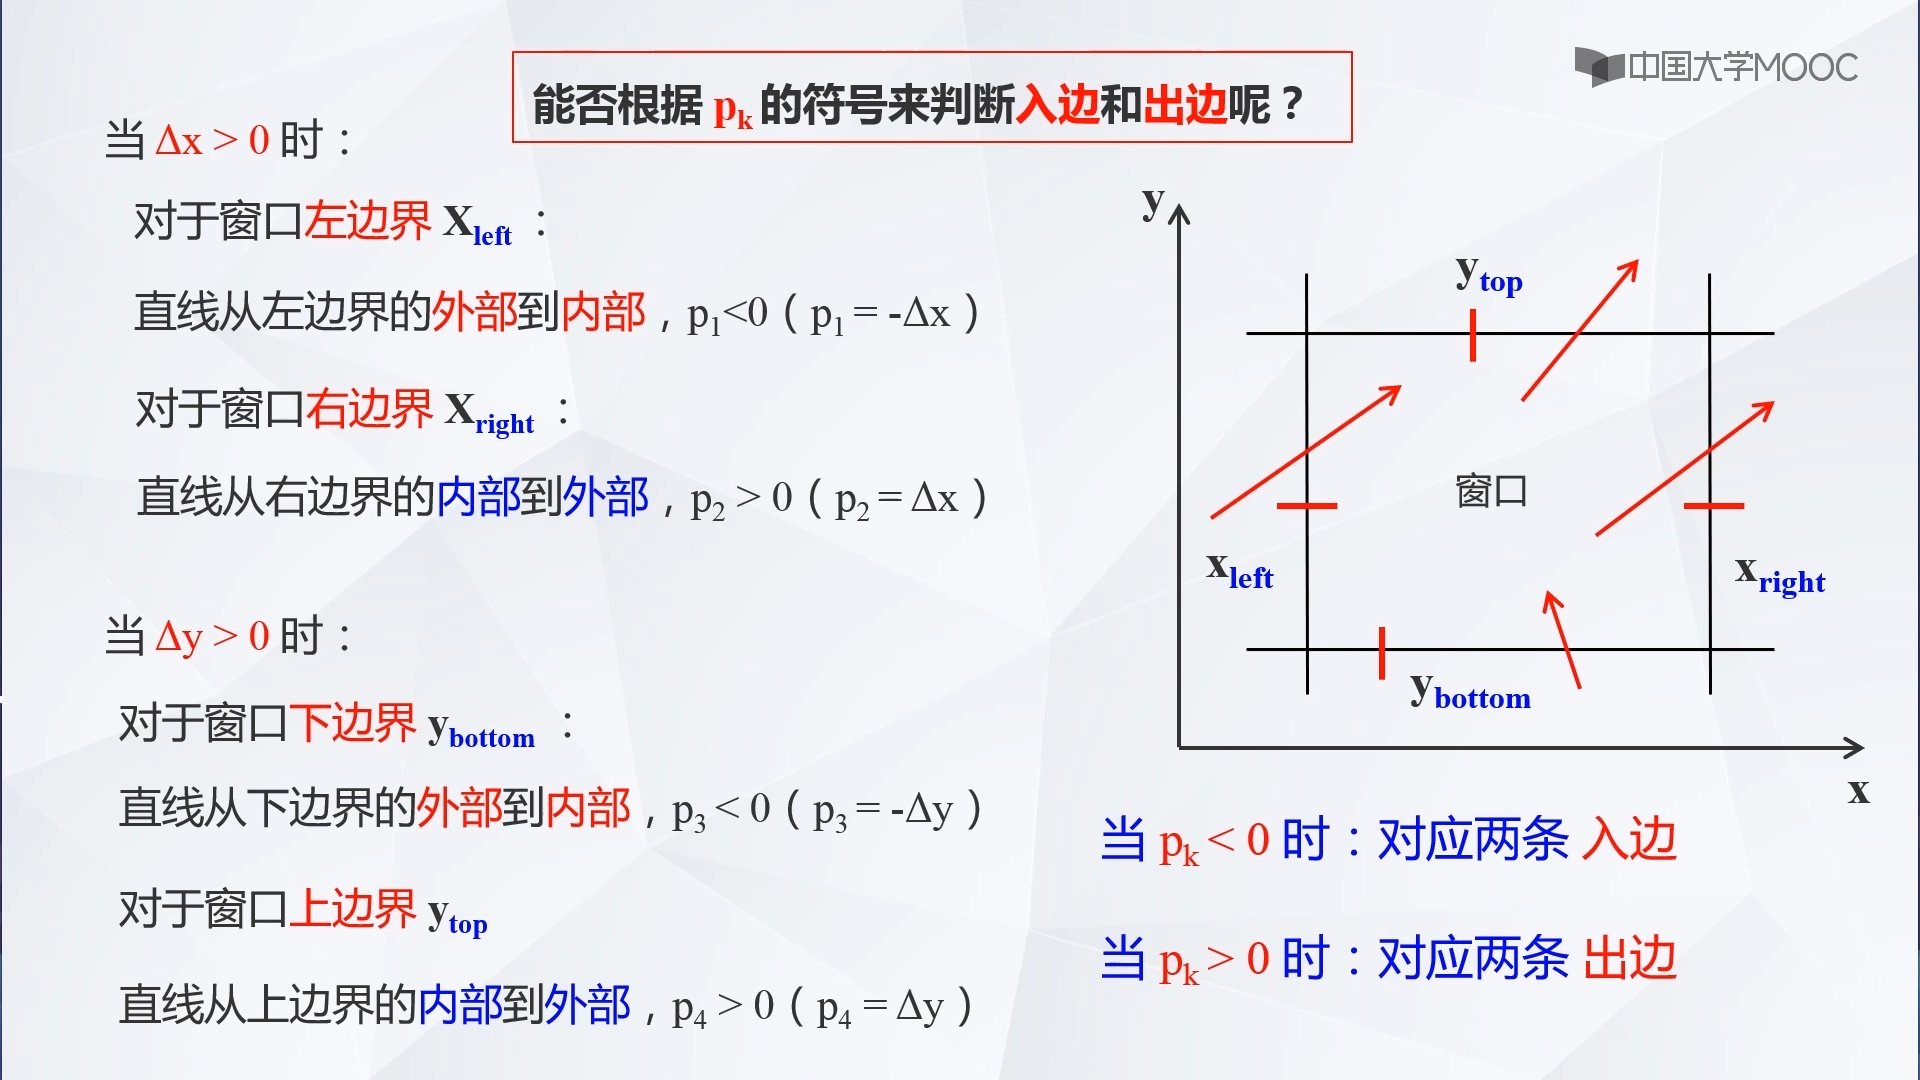
\includegraphics[scale=0.2]{figure/example.png}
	\caption{梁友栋-Barsky算法示意图}
	\label{fig:Barsky}
\end{figure}
对应的使用了好几个变量,包括 $\delta x$表示的是直线左右上的方向
然后对应的$\delta y$ 上下的方向。具体的公式如下\\
$$
\begin{cases}
    p1 = - \Delta x \\
    p2 = \Delta x\\
    p3 = - \Delta y \\
    p4 = \Delta y\\
    q1 = x_{1} - x_{left} \\
    q2 = x_{right} - x_{1}\\
    q3 = y_{1} -y_{bottom} \\
    q4 = y_{top} - y_{1}\\
\end{cases}
$$
对应的对上述的参数的数值进讨论可以得到线段和裁剪窗口的相对的位置关系

\begin{itemize}
    \item [(1)] 
    若pk=0,直线平行于裁剪边界之一。此时,如果同时满足qk<0,则线段完全在
    边界外;如果同时满足qk≥0,线段平行于裁剪边界,并且在窗口内;这种情况是相对简单一些的情况
    \item [(2)]
    当pk<0, 线段从裁剪边界延长线的外部延伸到内部
    \item [(3)]
    当pk>0,线段从裁剪边界延长线的内部延伸到外部
  \end{itemize}

对应的算法伪代码
\begin{itemize}
    \item [(1)] 
    将线段交点的参数初始化为 u1=0,u2=1;
    \item [(2)]
    定义一个函数,用 p、q 来判断是舍弃线段还是改变交点的参数r:
    当p<0 时,参数r 用于更新u1;
    当p>0 时,参数r 用于更新u2:
    如果更新u1 或u2 后使u1>u2,则舍弃该线段;
    否则,更新适当的u 值仅仅求出了交点,缩短线段。
    \item [(3)]
    p、q 的四个值经过测试后,当p=0 且q<0 时,说明该线段平行于边界且位于边
    界之外,舍弃该线段。假如该线段未被舍弃,则裁剪线段的端点由u1、u2 值决定。
    \item [(4)]
    反复调用算法进行计算
  \end{itemize}

使用下述的指令文件进行测试:\\

resetCanvas 600 600\\

setColor 0 255 0\\

drawLine line1 0 0 500 250 DDA\\

setColor 255 0 0\\

drawLine line2 0 0 500 250 Bresenham\\

translate line2 0 50\\

clip line2 50 50 400 200 Liang-Barsky\\

drawPolygon polygon4 50 50 400 50 400 200 50 200 Bresenham\\

saveCanvas 1\\

最后的测试结果

\begin{figure}[h]
	\centering
	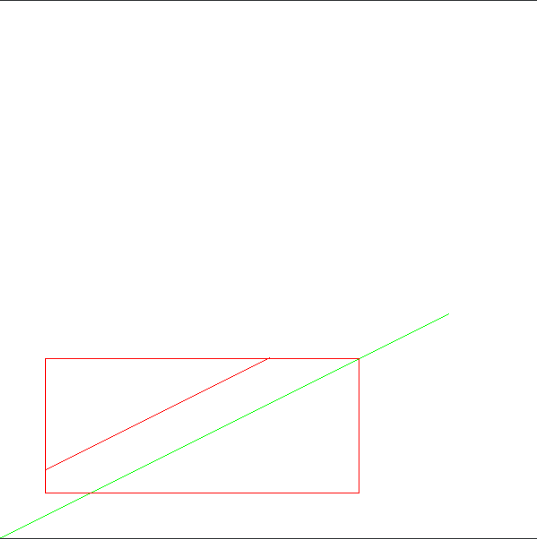
\includegraphics[scale=0.4]{figure/clip1.png}
	\caption{Liang-Barsky算法测试结果}
	\label{fig:Liang-Barsky算法剪切}
\end{figure}

\section{系统介绍}
目前的CG2020图形学系统已经支持
\begin{itemize}
    \item 命令行和GUI界面调用直线生成算法
    \item 命令行调用多边形生成算法和中点圆生成算法
    \item 在GUI界面中使用鼠标直接的选中所需图元
\end{itemize}

\section{总结}
本次实验基本还是以摸清框架代码结构以及了解QT特性为主,实现的代码量并不大
主要是实现了相对简单明了的直线生成算法以及相对复杂的多边形和中点圆生成算法,同时实现了图片检验模块,为后续的复杂
图像生成的正确性检验做一些准备,最后实现的鼠标选中图元的操作,即是方便操作
同时也是方便于后续复杂图元生成的时候测试和调试工作


\section{综述}
注:本次报告是增量式的报告,即本次的报告内内容就是这个月做的内容,不包含上个月已经报告过的任何内容

\begin{enumerate}
    \item 实现Bezier曲线绘制算法
    
    \item 实现B-Spline曲线绘制算法
    
    \item 在CLI做对应的处理,加入曲线绘制算法的对应功能

    \item 实现对图元的平移,旋转,缩放以及裁剪的操作,至此已经实现了所有算法模块里的内容
    
    \item 对CLI中添加对图元操作的相关支持
\end{enumerate}



\section{系统介绍}
目前的CG2020图形学系统已经支持
\begin{itemize}
    \item 命令行和GUI界面调用直线生成算法
    \item 命令行调用多边形生成算法和中点圆生成算法
    \item 在GUI界面中使用鼠标直接的选中所需图元
    \item 命令行调用曲线生成算法,可选算法Bezier和B-spline
    \item 在命令行调用指令,对图元做平移,旋转,缩放,裁剪操作
\end{itemize}

\section{总结}
本次实验基本是在实现和完善算法模块,集中对需求的图形学绘制和图元操作算法
进行研究和实现,至此已经实现了所有的算法函数,下一步是更加细致的查错和
完善在GUI里对算法的调用和支持



\section{综述}
注:本次报告是增量式的报告,即本次的报告内内容就是这个月做的内容\\
在上个月已经基本实现了算法部分的内容,这个月的工作主要可以概括到下面的四个方面
\begin{enumerate}
    \item 着手阅读GUI的框架代码
    
    \item 着手阅读pyQT相关的模块和接口
    
    \item 着手实现GUI相关的功能
    
    \item 修改遇到的算法模块的BUG
\end{enumerate}

目前已经实现的GUI部分
\begin{enumerate}
    \item 绘制直线,椭圆,多边形。
    
    \item 利用鼠标选中图元
    
    \item 平移,旋转
    
    \item 保存和清空画布
    
    \item 选择画笔颜色
\end{enumerate}
\section{GUI框架介绍}
\subsection{概述}
GUI框架主要是由如下的三个部分组成的

\begin{enumerate}
    \item MyCanvas:主要是画布,负责管理各个图元以及和监管鼠标的操作,会根据鼠标
    的操作已经当前的状态做对应的反应
    
    \item MyItem:作为基本的图元单位,保存了图元的信息以及图元的最基本的操作
    比如绘制自己和他的选中框
    
    \item MainWindow:作为相对上层的一个结构,主要负责的就是管理下游的图元
    更多的他代表了外层的窗口管理,负责和一些鼠标对菜单的操作的响应
\end{enumerate}

\subsection{具体函数分析}
\subsubsection{MyCanvas}
start\_draw\_line类似的函数主要就是负责绘制,但是这里的绘制并不是真正的绘制
在画布上的绘制,而是开始准备绘制色湖之状态位,在每一次的刷新才会根据Item自己的操作
进行绘制和显示。

以mouse打头的操作一般都是上文提到的对鼠标的操作进行响应的操作,包括鼠标的按下
移动以及松开,对应的在绘制里就是开始记录坐标点的时机。对于鼠标的按下还需要根据当前的
状态看看是不是选中图元之类的操作

\subsubsection{MyItem}
最基本的图元单位,保存了图元的相关信息,这里并不是直接保存了所有的绘制点,而是
保存了图元绘图的所需信息,即前面实现算法的时候需要的参数

有了上面保存好的参数之后就可以开始绘制,其中paint函数会做相关的操作,主要
的操作就是对每一个像素点draw,这个和QGraphicItem的内置有一些关系。

然后每一次除了画出自身之外还要记得看看自己是不是被选中了,如果是被选中的记得要把选中
框也要画出来,同时观察到这里绘制选中框设置设置了画笔的颜色,对应的可以实现
需求里的设置画笔的功能

\subsubsection{MainWindow}
这个类继承了QMainWinodow,同时在一开始的init里就有大量的设置的操作。
基本是在构造窗口的结构,以及设置按钮和绑定按钮和函数,涉及到了一些信号槽的
理念,此处略过。

各种以Action结尾的函数是作为按下按钮后的对应执行函数,主要做的事就是在和窗口
交互以及位Canvas的操作提供条件,基本的事件总结一下就是设置一下状态栏显示的
文字,然后调用对应canvas执行操作



\section{具体实现}
上面的解释是初步的在实现之前对框架代码的阅读理解,下面是具体的开发

\subsection{绘制直线}
对直线的绘制是相对简单的,因为有一个Naive作为基础,只需要类比,把
各种的函数调用换一下就行,这里省略不赘述,具体的实现思路和下面对于
椭圆绘制的实现相似

\subsection{绘制椭圆}
椭圆的绘制,根据日常的使用可以知道,在GUI里的期望动作就是可以点击鼠标,然后拖动
鼠标,鼠标停下的位置和一开始点击的位置是两个边界点,最终的椭圆就生成于这两个点
之间,同时在拖动的过程里可以看到椭圆变大变小从而便于观察和调整绘制的大小

所以结合之前对代码的观察,主要的实现步骤如下
\begin{enumerate}
    \item 增加椭圆相关的信号槽绑定
    
    \item 在MainWindow里添加相关的Action函数
    
    \item 进一步的就跳转到了start\_draw\_ellipse,把当前的状态设置好,然后选中
    当前的id,由于椭圆只有中点圆绘制一种算法,所以不需要指定算法的参数设定

    \item 接下来自然用户会开始操作鼠标,准备绘制,于是对应的在mousePressEvent
    函数中实现对应的功能,按下鼠标说明用户铁了心要画椭圆,于是根据刚才的状态
    进行判断,认为要画椭圆则生成对应的图元单位,然后放在列表里

    \item 刚才提到了随着鼠标的移动,待定的椭圆也要跟着变化,同时谁也不知道用
    户什么时候就不动然后松开鼠标,所以每次鼠标的移动都要保存下最后的位置,也就是
    把控制点(plist)的第二点设置为移动的位置,则代码就会做当前位置的绘制
    
    \item 截至到这里,基本椭圆的绘制GUI实现就已经做好了,其他的细节略
\end{enumerate}

\begin{figure}[h]
	\centering
	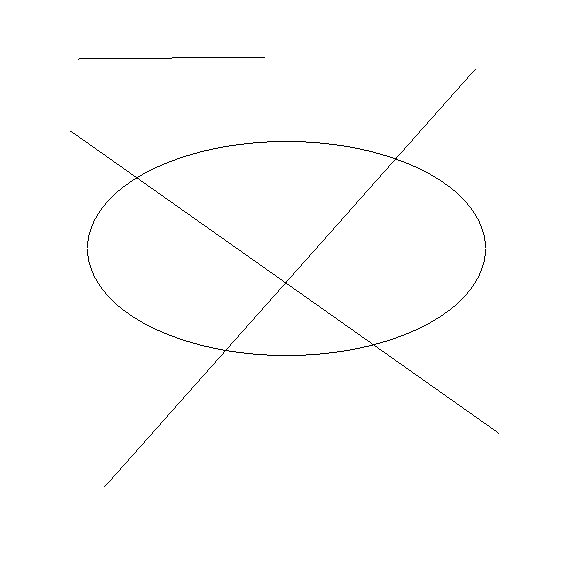
\includegraphics[scale=0.3]{figure/EillpsGUI.png}
	\caption{EillpsGUI效果图图}
	\label{fig:EillpsGUI}
\end{figure}


\subsection{绘制多边形}
多边形的绘制相对的会复杂一些,多边形是由多条边组成的,初步的设计是让鼠标的左键
不断的点击(拖动)选中新坐标点,然后鼠标右键表示作画结束,因此基本的实现思路就是
不断的捕获左键的操作,然后把坐标点加入p\_list。

注意到在作画结束之前,图形不一定是封闭的,于是原先写好的多边形绘制算法并不能
直接使用,因此对应的做了一些修改,封装到draw\_polygoning函数,取消了最后一个
点和第一个点的练接,直到捕获到右键之后说明作画结束,才会调用原来的绘制多边形函数

\begin{figure}[h]
	\centering
	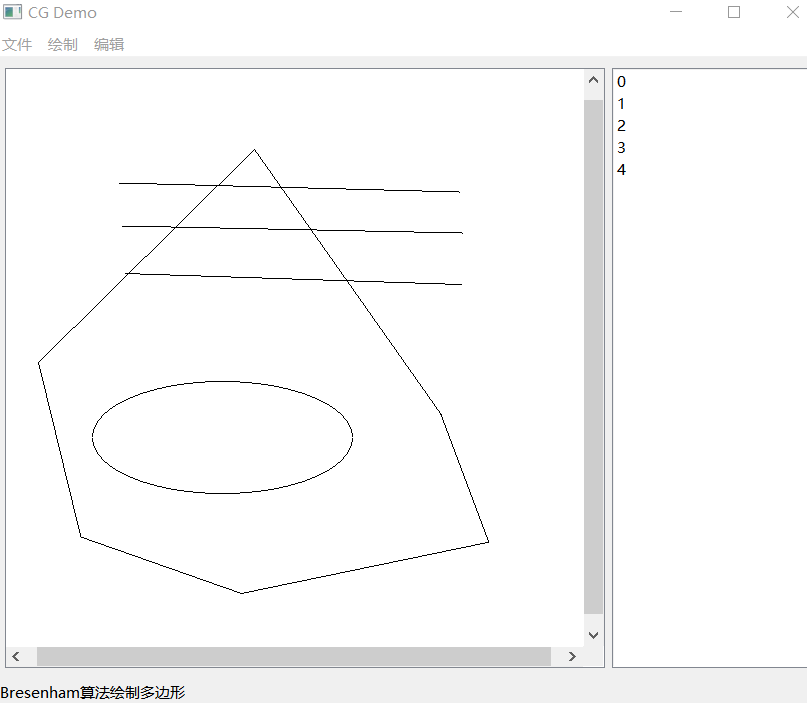
\includegraphics[scale=0.4]{figure/draw.png}
	\caption{绘图算法效果图}
	\label{fig:DrawGUI}
\end{figure}

\subsection{画笔设置}
之前已经提到了,框架代码在绘制的时候加上了设置颜色的操作,同理我可以在一开始的
时候设置在菜单里让用户选择对应的颜色,等到用户选择好了颜色之后,我在类里加上
一个变量专门记录一下这个选择的结构,然后在Item每一次绘制的时候都提醒Item使用
对应的颜色作画。

实现流程实际上和上述实现椭圆的过程是差不多,都是要从MainWindow开始入手,先
修改菜单的结构,然后Connect信号和槽,接着在Canvas里和item里对应实现即可,自身
没有太大的技术需求

比较有意思的就是用到了Qt提供的一个QColorDialog,能够直接显示出选择颜色的颜色盘

\begin{figure}[h]
	\centering
	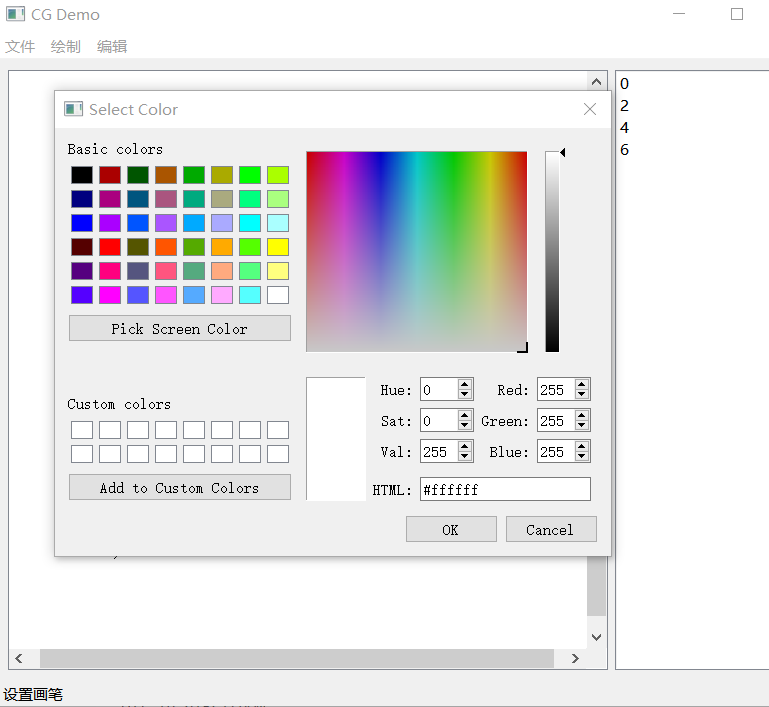
\includegraphics[scale=0.3]{figure/ChooseColor.png}
	\caption{设置画笔效果图}
	\label{fig:EillpsGUI}
\end{figure}


\subsection{保存图元}
实现保存图元,基本的操作和上面都是一样的,从定义菜单到槽函数等等
比较不一样的自然就是保存,怎么才可以把所有的绘制图元拔下来放进图片?
使用的是QGraphicsView里的grab来保存。然后QT中dialog提供了选择文件保存的
界面接口对话框:dialog.getSaveFileName。最后的实现效果基本如下

\begin{figure}[h]
	\centering
	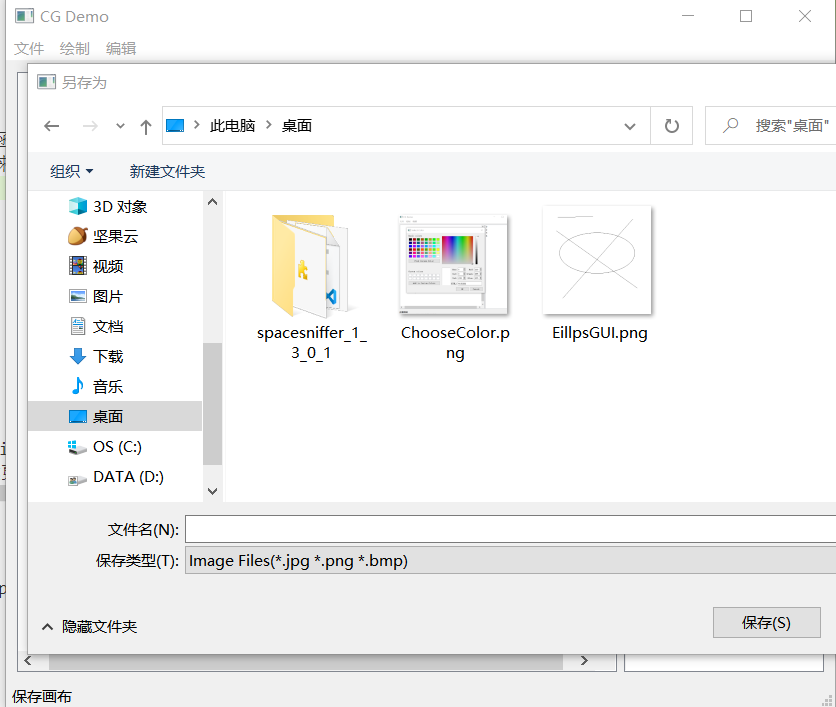
\includegraphics[scale=0.5]{figure/SaveCanvas.png}
	\caption{保存界面示意图}
	\label{fig:SaveCanvas}
\end{figure}

以及最后保存的结果(输入的文件名就是test)
\begin{figure}[h]
	\centering
	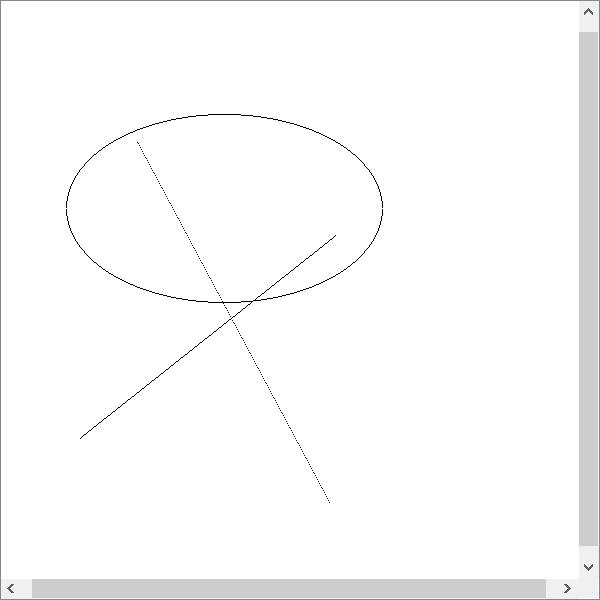
\includegraphics[scale=0.5]{figure/test.jpg}
	\caption{保存画布结果图}
	\label{fig:SaveCanvas}
\end{figure}

\subsection{BUG修复}
在进一步的实现GUI的时候发现了一些BUG,随后进行了修复

\subsubsection{曲线绘制算法BUG}
之前的曲线绘制没有考虑到左右两个端点是同一个点的情况,同样在测试样例里也没有这样
但是在GUI的使用的时候,由于椭圆是随着鼠标的移动而绘图的,所以这个时候一开始会出现左右两个端点在同一个位置的情况
进一步的触发了BUG,发现这个BUG后进行修改,在计算之前就先加入左右端点即可

 
\section{系统介绍}
目前的CG2020图形学系统已经支持
\begin{itemize}
    \item 命令行和GUI界面调用直线生成算法
    \item 命令行调用多边形生成算法和中点圆生成算法
    \item 在GUI界面中使用鼠标直接的选中所需图元
    \item 命令行调用曲线生成算法,可选算法Bezier和B-spline
    \item 在命令行调用指令,对图元做平移,旋转,缩放,裁剪操作
    \item 在GUI界面绘制直线,多边形,椭圆
    \item 在GUI界面操作图元平移
    \item 在GUI界面调整画笔
    \item 在GUI界面保存画布
\end{itemize}

\section{总结}
本次实验主要是对GUI的框架代码进行了相对深入的了解,在了解的同时
逐步的开展相应的功能实现,主要围绕着绘图和绘图相关的实用功能。
在实现的同时,检测和挖掘先前算法实现的种种BUG并修复
\bibliography{xxx}

\begin{thebibliography}{99}  
    \bibitem{ref1}《计算机图形学教程》孙正兴编 
    \bibitem{ref2} \href{https://www.google.com/imghp?hl=zh-CN&ogbl}{Google图片}
    \bibitem{ref3} \href{https://blog.csdn.net/shenziheng1/article/details/54411098}{CSDN博客}
    \bibitem{ref4} \href{https://build-system.fman.io/pyqt5-tutorial}{PyQT5 Tutorial}
\end{thebibliography}

\end{document}
\bibliographystyle{plain}
